\chapter{Computational Study}
\label{ComputationalStudyChapter}

% quote: model something

\begin{quote}

\end{quote}

\epigraph{You don't really understand what you've got until you do a comprehensive model of it}{\textit{Christopher Tyler - VSS 2019}}

In both the small and large sphere experiments an assumption was made that adapting to the periphery would affect foveal colour perception. This was not a particularly unreasonable assumption, considering that iprgcs are predominantly extra-foveal, whereas our finest perception of color is foveal.
It is an assumption nonetheless, and it was assumptions such as this (similar examples can be drawn regards the temporal and spectral choices we made) which drew me to consider a more abstract form of experimentation - experimental computational modeling.
Here I consisted my goal to be primarily a Marr's level 1 goal - to understand the challenge faced by the HVS, and consider whether a melanopain based signal might be valuable in the pursuit of colour constancy, given the conditions existent on planet earth, and the behavioral goals of a creature with a visual system.

%% - %%

\section{Introduction}

I am interested in the question of whether a melanopic signal might be useful for either estimating the illuminant(s) in a scene, or more directly transforming visual signals into an illuminant-independent space.

Following initial psychophysical experiments, where results did not indicate a strong or simple relationship, I chose to take a step back and examine the problem that the HVS is faced with in a natural environment, which colour constancy solves. Through this route I hoped to answer the questions:
\begin{enumerate}
	\item Would it be sensible for the HVS to use a melanopic signal to help solve this problem?
	\item If so, in what way would it be used?
\end{enumerate}

In this document I shall give an overview of the main scripts I have written, going through the logic and results of each.
All scripts are available at \url{https://github.com/da5nsy/Melanopsin_Computational}

\section{melcomp\_1}

In melcomp\_1 I set out with three questions:
\begin{enumerate}
\item Considering only daylight spectra (excluding reflective surfaces for now), can a melanopic signal predict the chromaticity of daylight more precisely than signals provided by other retinal cell populations?
\item Now considering also object reflectances, does a melanopic signal provide a means of calculating a sign and weight of shift required to counteract the chromatic shift induced upon objects by a change in daylight conditions?
\item Are there objects, or luminance levels, or daylight chromaticities for which the melanopic signal is particularly effective or ineffective at performing the above task
\end{enumerate}

The final question was asked with the hope that such limitations might provide nice tests to perform psychophysically. 

Foundational data consisting of the Granada daylight dataset, the Stockman-Sharpe 10 degree cone fundamentals, the Lucas et al. melanopsin fundamental, and the a subset of the Vrhel et al. reflectances (consisting of the `natural' reflectances) were used.

Tristimulus values $[L,M,S]$ and analogous melanopic values ($I$) were calculated for each illuminant within the Granada dataset. The real-world correlate of this computation would be to observe a spectralon tile under each daylight condition.

\ac{MB} chromaticity co-ordinates were calculated, and three-dimensional plots were made to display $l_{\text{MB}}$ against $s_{\text{MB}}$ against $[L,M,S,I]$ in turn. Each plot is shown in \ref{fig:l1}. As can be seen, although there exists some relationship between the chromaticity values and the first level values, it does not appear as though one could predict the other. All that can be said from this relationship is that if the first level value is above a certain threshold, it is likely to be in a group with a low $s_{\text{MB}}$ value. The real-world correlate of this is to say - \textit{if the day is bright enough, I can be fairly confident that the chromaticity of daylight will be relatively warm in colour.} This is as expected, since the brightest daylight conditions are likely to be those with unobstructed direct sunlight, which is warmer in colour than illumination provided by the blue sky. This relationship seems relatively weak however, and could not be used to accurately predict the chromaticity of an illuminant. The answer to the first question set out for the script then, is that a melanopic signal cannot predict chromaticity (though neither can any other signal).

\begin{figure}[h]
    \centering
    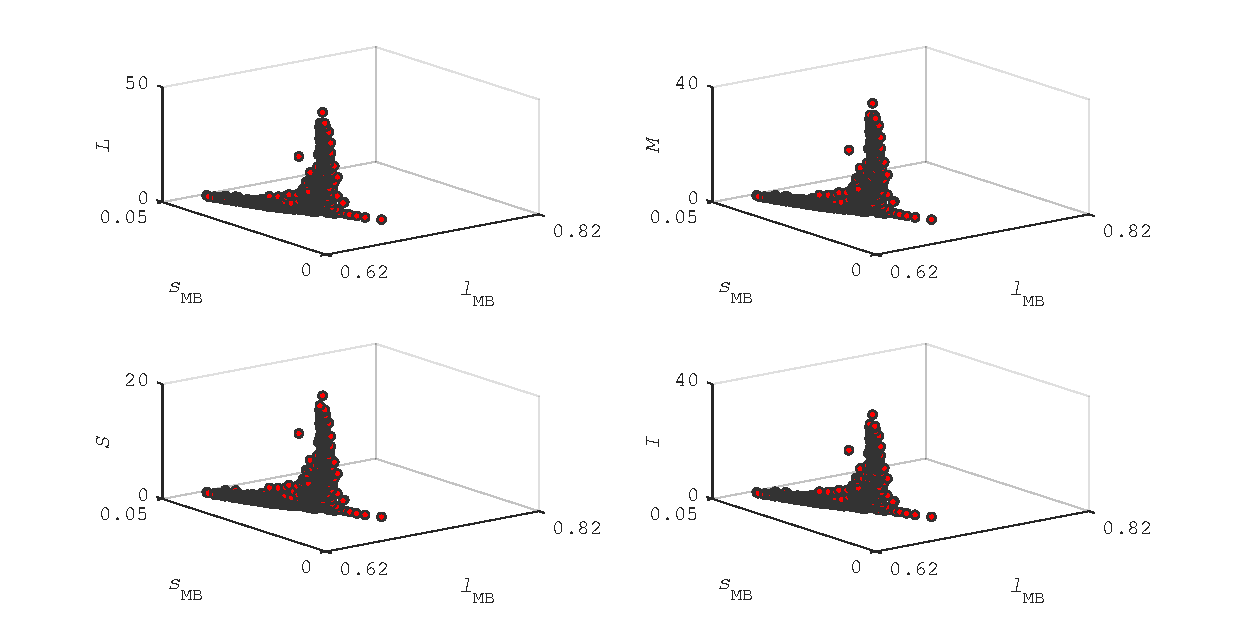
\includegraphics{C:/Users/cege-user/Dropbox/Documents/MATLAB/Melanopsin_Computational/figs/melcomp_1/level1sigspredictingColorimetry.pdf}
    \caption{\hl{Caption}}
    \label{fig:l1}
\end{figure} 

\begin{figure}[h]
    \centering
    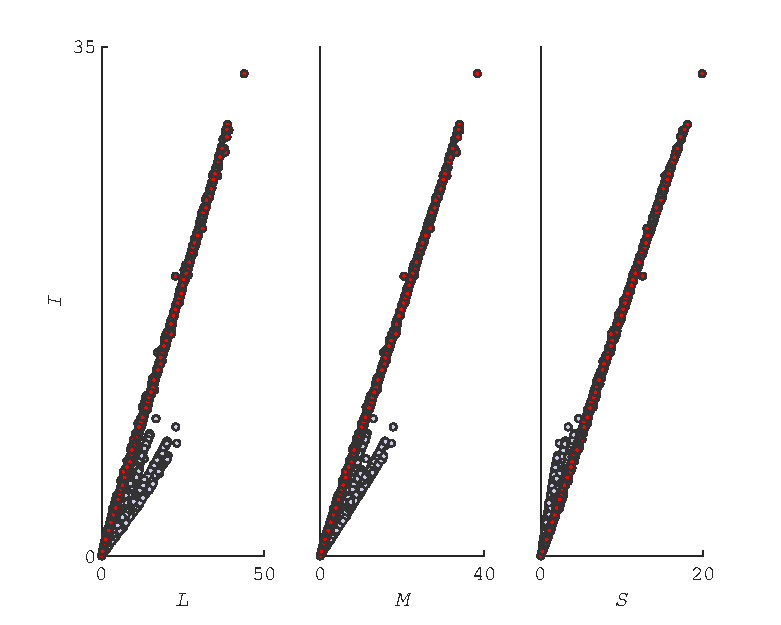
\includegraphics{C:/Users/cege-user/Dropbox/Documents/MATLAB/Melanopsin_Computational/figs/melcomp_1/correlationBetweenLevel1Sigs.pdf}
    \caption{The relationship between melanopic power (analogous to a tristimulus value but calculated using the spectral sensitivity of melanopsin) with the traditional tristimulus values showing a strong correlation. Red points indicate signals computed directly from the spectral power distribution, grey points represent values of computed colorimetry for objects under illuminants.}
    \label{fig:tristimCorrelation}
\end{figure} 

It should be noted that there was very high correlation between each signal. This can be considered as corresponding to the high importance of the first principal component of the spectral measurements in this dataset. Put another way, a sensor with almost any spectral sensitivity could be used to estimate the magnitude of the daylight. I shall return to the discussion of principal components when discussing melcomp\_3.

\begin{minipage}{\linewidth}
\begin{lstlisting}
corr(LMSM')

    1.0000    1.0000    0.9993    0.9998
    1.0000    1.0000    0.9995    0.9999
    0.9993    0.9995    1.0000    0.9999
    0.9998    0.9999    0.9999    1.0000
\end{lstlisting}
\end{minipage}

Following this, similar plots were made which plotted $l_{\text{MB}}$ against $s_{\text{MB}}$ as before, but now plotted the various combinations of $[L,M,S,I]$ created by considering one signal over another (e.g. $L/M$). Following the terminology of \cite{barrionuevo_contributions_2014} I shall refer to $[L,M,S,I]$ as `first level signals' and these derived signals as `second level signals'. The twelve plots created all showed clear and relatively simple relationships between chromaticity and these new derived signals.

For many of these signals however, such relationships are to be expected. For example, a relationship between $l_{\text{MB}}$ and $L/M$ should be expected, since $l_{\text{MB}}$ is defined as the sum of weighted components of $L$ and $M$. To confirm this, a null condition was performed, where $[L,M,S,I]$ was replaced by randomly generated values, and the second level signals were generated as before. Relationships between secondary signals derived from L, M or S signals still showed correlations with chromaticity (albeit now points fell on a plane, instead of a line), whereas signals with a $I$ component showed only minimal coherence, forming a rough cloud in three-dimensional space. 

This example shows that a melanopic signal exhibits correlation with a chromatic signal \emph{not} due to the underlying mathematics of how chromaticity is calculated, and that any relationship must follow from a genuine regularity in the data.

Following this, reflectances were introduced, so as to consider a slightly more realistic situation. Now the simulation considered the colour signals produced by each of the recorded reflectances, under each of the recorded illuminants. \ac{MB} chromaticities, and an analogous melanopic signal, were computed as defined by equation \ref{eq:i} (see \cite{macleod_chromaticity_1979} and \cite{cie_cie_2015}), where $k_1$ and $k_2$ represent the constants required such that the sum of the weighted $L$ and $M$ signals equals or approximates the luminance function. Chromaticities are plotted in figure \ref{fig:mb}.

\begin{equation} \label{eq:i}
i_{MB} = I/(k_1L + k_2M) 
\end{equation}

\begin{figure}[h]
    \centering
    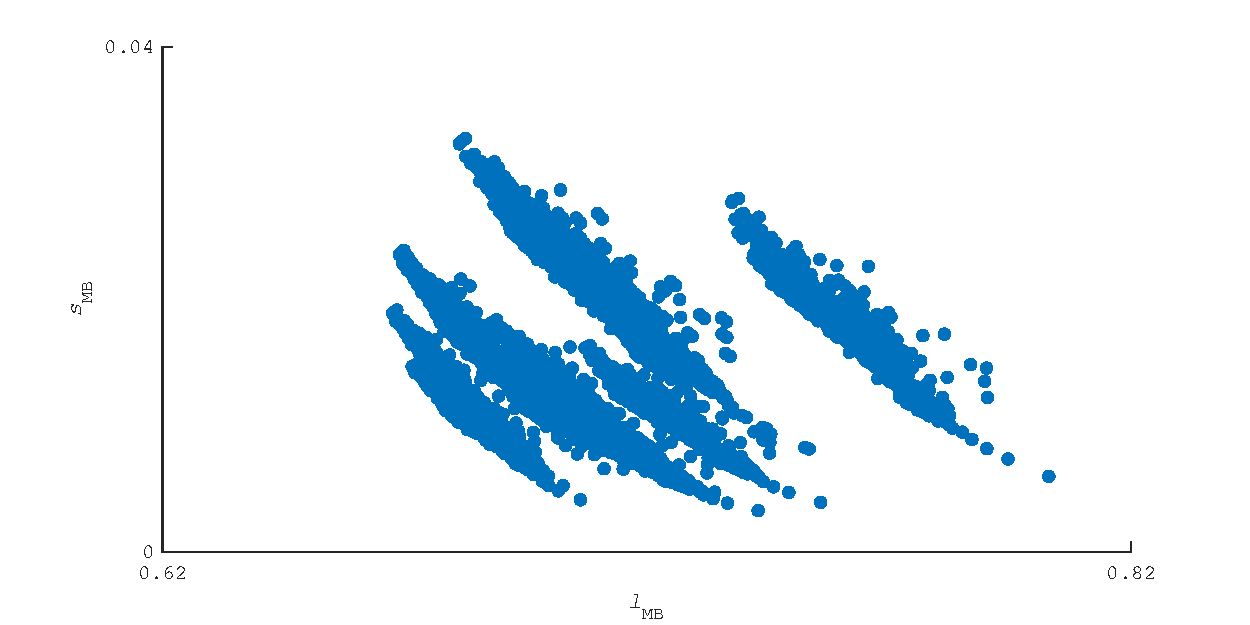
\includegraphics{C:/Users/cege-user/Dropbox/Documents/MATLAB/Melanopsin_Computational/figs/melcomp_1/BasicMB.pdf}
    \caption{\ac{MB} chromaticities for 12 reflectances under 2600 daylight illuminants.}
    \label{fig:mb}
\end{figure} 

Now able to consider the second question, I considered whether it was possible to perform a conversion of these computed chromaticities into a hypothetical illuminant-independent space, using $i_{\text{MB}}$ as a corrective signal. It was found through an optimization procedure that through addition and subtraction of weighted $i_{\text{MB}}$ values, using the scaling factors shown in equation \ref{eq:correction} such a conversion could approximately be performed. The results of applying equation \ref{eq:correction} can be seen in figure \ref{fig:corrected}.

\begin{subequations} \label{eq:correction}
\begin{align}
l_{\text{MB}}* &= l_{\text{MB}} + 0.23i_{\text{MB}}\\
s_{\text{MB}}* &= s_{\text{MB}} - 1.70i_{\text{MB}}
\end{align}
\end{subequations}

\begin{figure}[h]
    \centering
    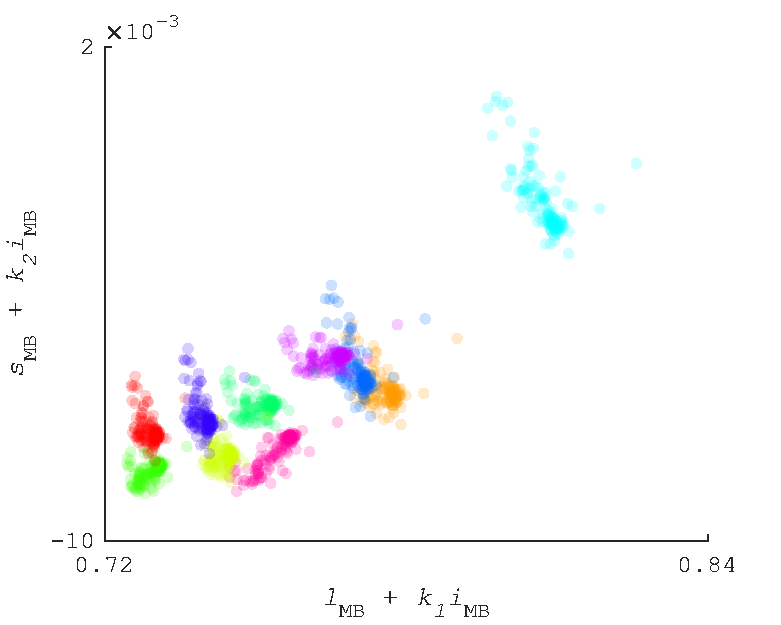
\includegraphics{C:/Users/cege-user/Dropbox/Documents/MATLAB/Melanopsin_Computational/figs/melcomp_1/correctedChromaticities.pdf}
    \caption{\ac{MB} chromaticities for 12 reflectances under 2600 daylight illuminants, corrected by the corresponding $i_{\text{MB}}$ value.}
    \label{fig:corrected}
\end{figure} 

It can be seen that the points now roughly cluster together by object, with less smearing induced by changes in illuminant.

Following this, an additional optimization procedure was performed, to consider whether shifting the sensitivity of the melanopsin function along the wavelength spectrum affected the performance of such a signal in correcting these values. The optimization sought to minimise the overall spread of chromaticities (measured as standard deviation of the entire set). The results of this optimisation can be seen in figure \ref{fig:opt}. It can be seen that minima for $l_{\text{MB}}$* occur at around 530nm and just under 600nm, and minima for $s_{\text{MB}}$* occur at around 450nm and 580nm. On first appearance this seems to suggest that the optimal spectral sensitivity for a cone type employed to correct the signals from the various cones might be around these points in the spectrum. However, the careful reader might note the correspondence between the figures above and the peak spectral sensitivities of the cones themselves (S-448nm, M-541nm, L-569nm). Indeed we see that the optimal performance occurs when the nominal melanopsin sensitivity overlaps most well with the spectral sensitivity of the cones. It is understandable why this occurs - each signal is then normalised by a near-duplicate of itself, rendering each value in the set being close to zero.

\begin{figure}[h]
    \centering
    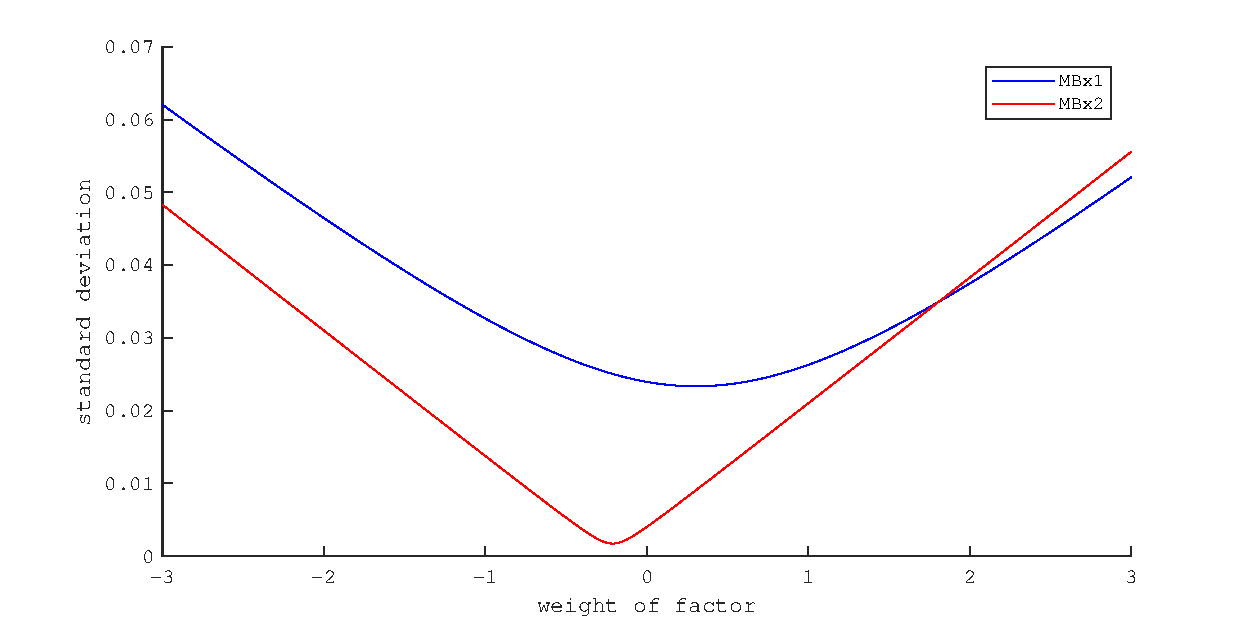
\includegraphics{C:/Users/cege-user/Dropbox/Documents/MATLAB/Melanopsin_Computational/figs/melcomp_1/minimiseSD.pdf}
    \caption{A plot showing the optimal minima for the factor weights.}
    \label{fig:minSD}
\end{figure} 

\begin{figure}[ht]
    \centering
    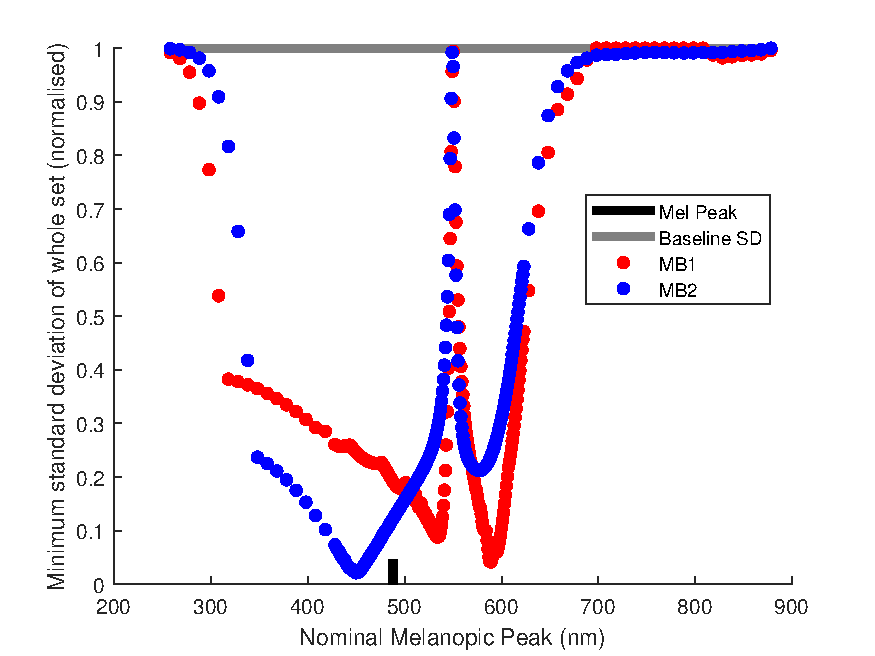
\includegraphics{C:/Users/cege-user/Dropbox/Documents/MATLAB/Melanopsin_Computational/figs/melcomp_1_caller/opt.pdf}
    \caption{The results of an optimization where the spectral sensitivity of the nominal melanopsin fundamental was shifted along the spectrum. Generated using melcomp\_1\_caller.m for iteration.}
    \label{fig:opt}
\end{figure} 

This had the unexpected and unfortunate effect of simply crushing all the chromaticties down onto a single line, without preserving any inter-object chromatic differences. We witness perfect colour constancy, at the expense of any chromatic discrimination. This is obviously not ideal.

\begin{figure}[h]
    \centering
    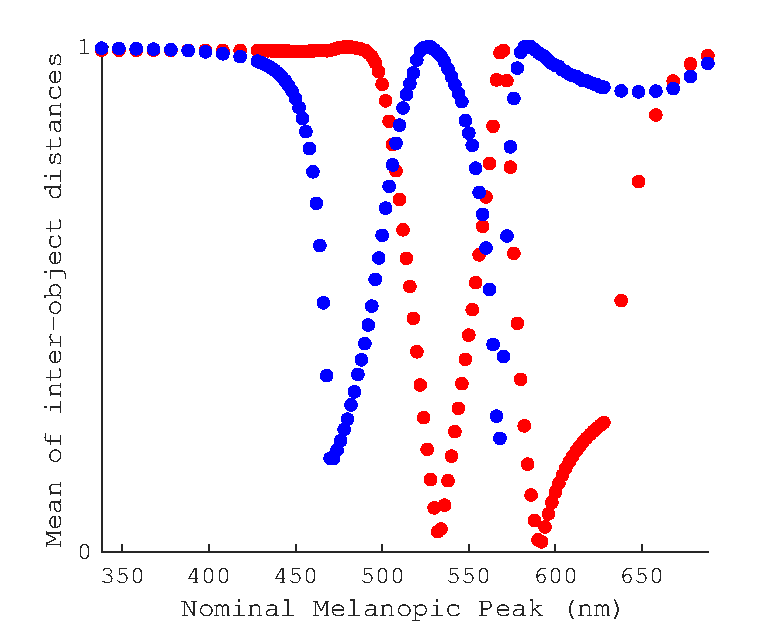
\includegraphics{C:/Users/cege-user/Dropbox/Documents/MATLAB/Melanopsin_Computational/figs/melcomp_1_caller/sdmeans.pdf}
    \caption{Normalised average distance between points in the set of the mean chromaticities for the different reflectances. It can be seen that inter-reflectance variation drops to zero at the same minima as seen in figure \ref{fig:opt}, showing that these distinct points are undesirably corrected to the same point. Generated using melcomp\_1\_caller.m for iteration.}
    \label{fig:sdmeans}
\end{figure} 

The work was presented at this stage as a poster at the \emph{Vision Science Society Conference (VSS)} in 2018, which is available at \url{doi.org/10.6084/m9.figshare.6280865}.

The actual desired behaviour would be to minimise internal variance for each reflectance group, whilst maintaining at least some distinction between inter-reflectance groups. A comprehensive approach to this question would need to consider the relative importance of the two separate requirements, and apply appropriate weightings.

\hl{Conclude with answers to the 3 initial questions}

\section{melcomp\_2}

Following VSS I changed my perspective on the problem slightly and started thinking about the $i_{\text{MB}}$ signal as a third dimension upon the already two-dimensional \ac{MB} chromaticity space, such as shown in figure \ref{fig:ZL}. This allowed me to consider what properties a signal upon this third dimension would need to provide to the overall three-dimensional point cloud in order for a transformation to occur which would transform the values into a two-dimensional illuminant-independent space.

\begin{figure}[h]
    \centering
    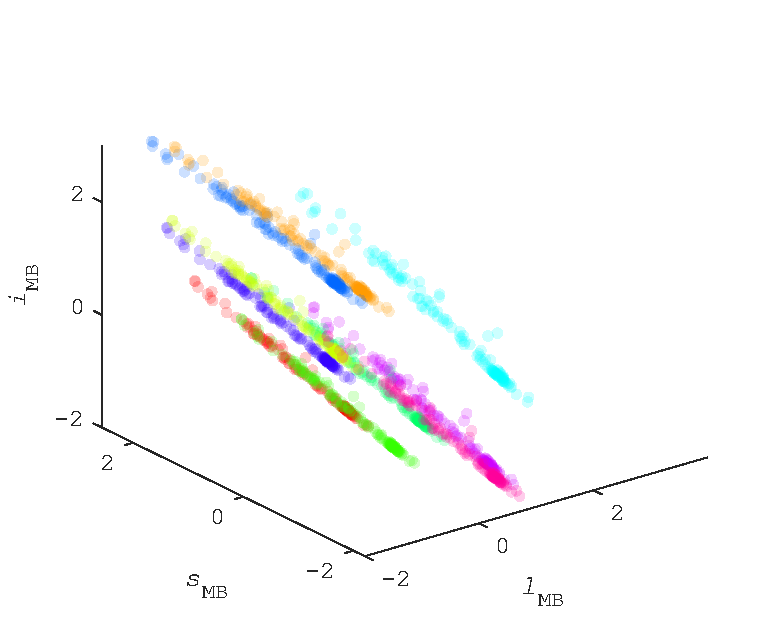
\includegraphics{C:/Users/cege-user/Dropbox/Documents/MATLAB/Melanopsin_Computational/figs/melcomp_2_figs/ZL.pdf}
    \caption{\hl{caption}}
    \label{fig:ZL}
\end{figure} 

The script started with the same process as melcomp\_1, loading data and computing \ac{MB} chromaticities, along with hypothetical $i_{\text{MB}}$ values. $r_{\text{MB}}$ values, the rod based analogue, were also calculated, although this was done for completeness (again, following the influence of \cite{barrionuevo_contributions_2014}) rather than following a genuine belief that they could be involved.

In addition to the data considered in melcomp\_1, support was added to consider a range of CIE D series illuminants, the Foster et al. hyperspectral images of natural scenes and the Smith-Pokorny fundamentals.

The CIE D-series illuminants allowed for a smaller and more controlled dataset, the Foster et al. data allowed for a more realistic distribution of reflectances and the Smith-Pokorny fundamentals allowed for a technically `correct' \ac{MB} diagram (before I knew about CIE 170-2:2015 \cite{cie_cie_2015}).

The key finding at this stage was that there is a perspective upon a three-dimensional point cloud ($[l_{\text{MB}},s_{\text{MB}},i_{\text{MB}}]$) from which points from like objects clustered well, such as in figure \ref{fig:viewpoint}. This property shows that there is at least one transformation such that the points could be projected upon a two-dimensional plane where the illuminant dependence was greatly reduced whilst the inter-object chromatic relationships were retained. 

\begin{figure}[h]
    \centering
    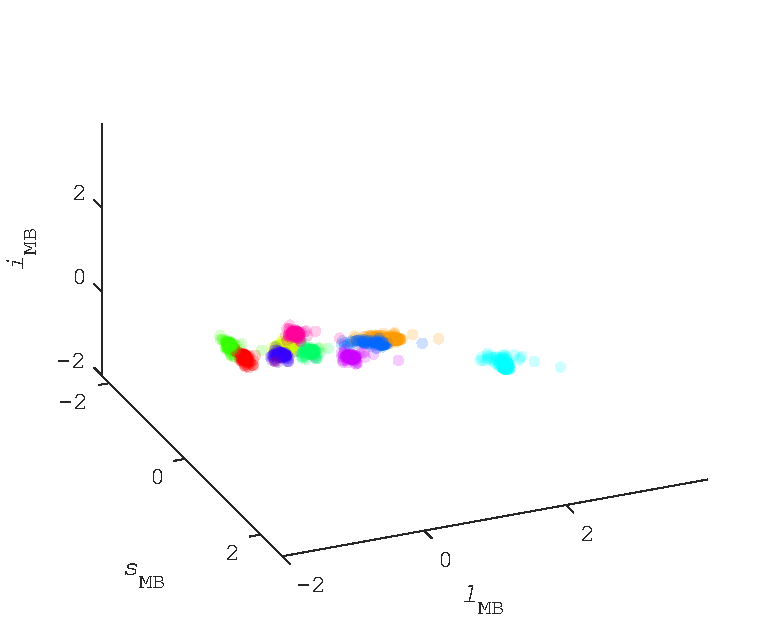
\includegraphics{C:/Users/cege-user/Dropbox/Documents/MATLAB/Melanopsin_Computational/figs/melcomp_2_caller/viewpoint.pdf}
    \caption{Figure \ref{fig:ZL} rotated to a perspective where it can be seen that the points project upon a two-dimensional plane in a clustered fashion whilst not degrading to a line within that space.}
    \label{fig:viewpoint}
\end{figure} 

Note that such a perspective would not be possible for a space where the third dimension were a duplicate of the first or second, since in this case all points would lie upon a plane. This would be the case in circumstances where a corrective signal too closely resembled the visual signals.

Following this, a range of speculative transformations were performed, to demonstrate the types of transformation that could be used to transform colour signals to illuminant-independent colour signals. A rotational transformation was successful (analogous to changing the perspective as in figure \ref{fig:viewpoint}) and additionally a weighted additive model was found to be more-or-less successful. No satisfactory model was found where a purely multiplicative transformation was applied.

Thinking about a corrective signal as an additional dimension upon a \ac{MB} chromaticity space allows for consideration of requisite or desirable properties that this third signal should imbue upon the three-dimensional cloud of points. I have identified one requisite property, and one desirable property. 

The requisite property for such a signal, as already suggested, is that it should differ from other chromatic signals enough to allow for the point cloud of chromatic points to be significantly \emph{non-planar}. This in turn allows for a projection upon two-dimensional space which has the potential to be illuminant-invariant.

The desirable property is that it should be \emph{roughly monotonic} with respect to other chromatic signals. This allows a one-to-one mapping of colour signals to illuminant-independent colour signals, where a non-monotonic relationship does not necessarily do so. This is not a strict requirement, since the corrective function only needs to be one directional, but non-monotonicity would exclude simple transforms (such as linear additive or rotational).

The next stage was to search for the underlying reason for the relative success of these transforms. One potential lead is a curious regularity at the lower wavelengths of the reflectance spectrum of many natural objects. In figure \ref{fig:plateau} it can be seen that there is a plateau in the relative spectral reflectances of some natural objects (a subset of the Vrhel reflectances) between roughly 430nm and 480nm, with relatively small deviations within 400nm to 500nm. Another way to visualise this is to calculate the correlation between points on the reflectance function. Such a calculation was performed initially on the Foster data, and then on three other datasets. See figure \ref{fig:foster} and \ref{fig:others} respectively.

\begin{figure}[h]
    \centering
    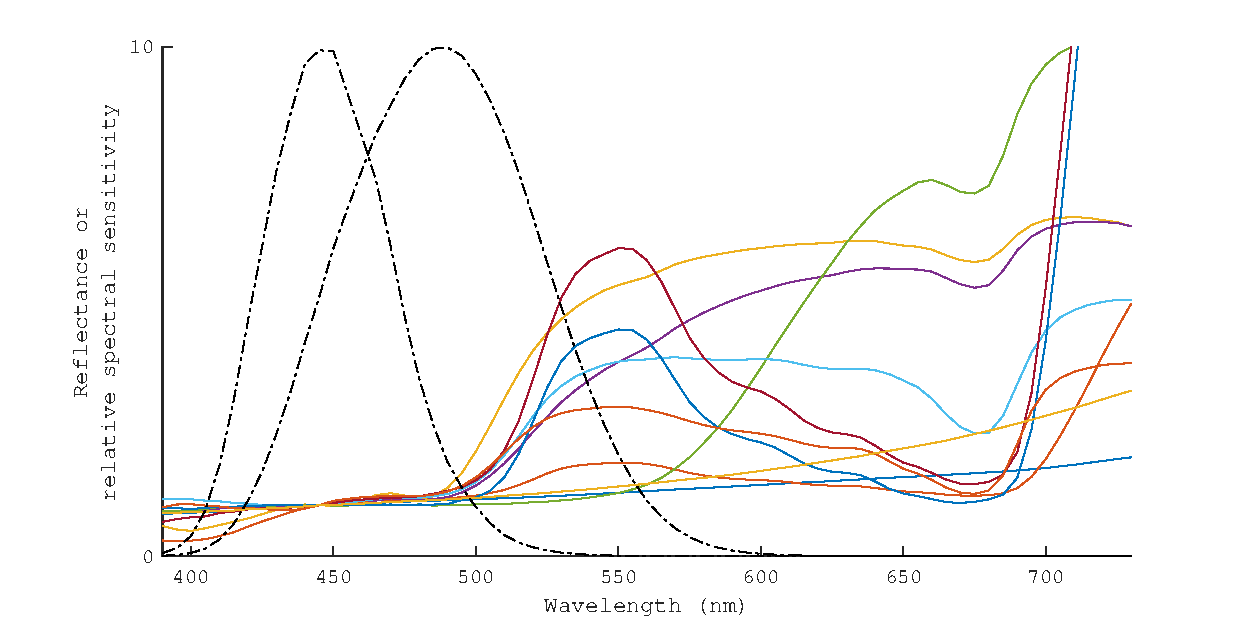
\includegraphics{C:/Users/cege-user/Dropbox/Documents/MATLAB/Melanopsin_Computational/figs/melcomp_2_caller/plateau.pdf}
    \caption{The spectral reflectance functions of a subset of the Vrhel reflectances (solid lines), normalised at the peak of s-cone sensitivity, with the spectral sensitivity of s-cones and melanopsin overlaid (dot-dashed lines).}
    \label{fig:plateau}
\end{figure} 

\begin{figure}[h]
    \centering
    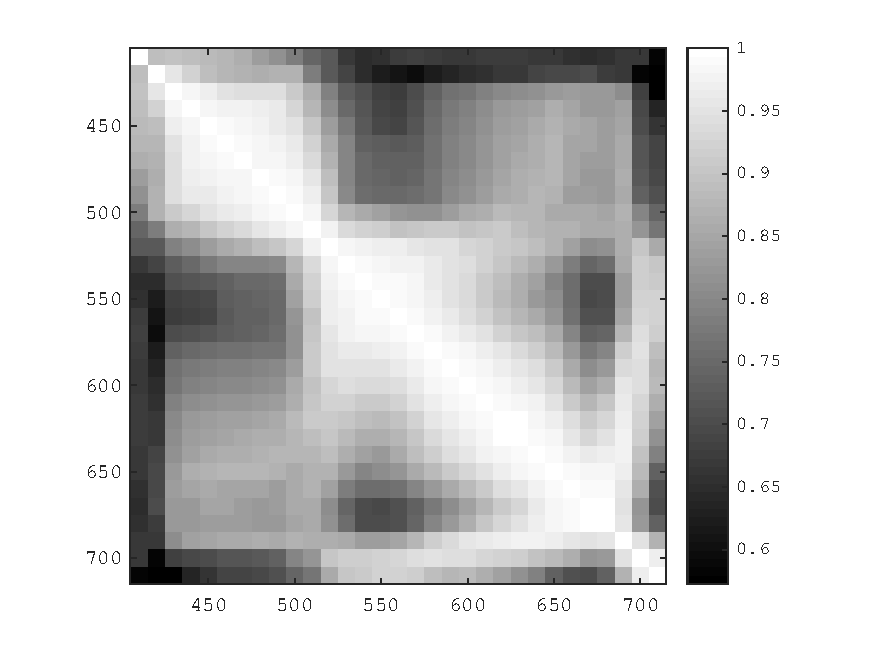
\includegraphics{C:/Users/cege-user/Dropbox/Documents/MATLAB/Melanopsin_Computational/figs/nat_cor/foster.pdf}
    \caption{\hl{caption}}
    \label{fig:foster}
\end{figure} 

\begin{figure}[h]
    \centering
    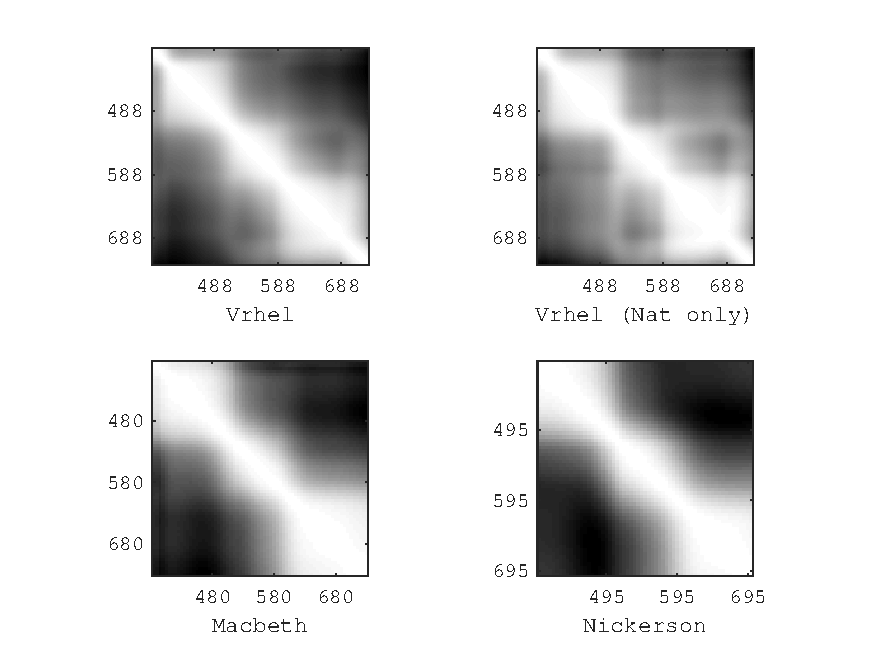
\includegraphics{C:/Users/cege-user/Dropbox/Documents/MATLAB/Melanopsin_Computational/figs/nat_cor/others.pdf}
    \caption{\hl{caption}}
    \label{fig:others}
\end{figure} 

An interesting advantage could be made of this regularity. Assume a simpler situation where there were two points on the spectrum of the reflectance functions of a set of natural objects which were always the same as eachother (perfect correlation). Sensors of appropriately narrow spectral sensitivity, placed at these two points on the spectrum would always register corresponding signals. Considering that the second principal component of daylight variability is a broad skew, any difference in the signals from two such receptors could be used fairly reliably to sense the contribution of this second component in any single condition. This explains the relative effectiveness of an $i_{MB}$ in correcting an $s_{MB}$ signal, but the logic for how it corrects an $l_{MB}$ signal is slightly trickier.

\hl{Note to LM: I think I've got it, but it will have to wait for the next draft!}

This work was presented as a poster at the \emph{Visual Neuroscience Summer School} in 2018 as a poster, which has not been made publicly available.

\section{melcomp\_3}

In melcomp\_3 I dove I approached the problem with a linear models approach, drawing on the work of Maloney \hl{refs!}. This is so far a bit of a bust, but I'm hoping that as I bring it all together it might click into place.


%\begin{figure}
%     \centering
%     \begin{subfigure}[b]{0.49\textwidth}
%         \centering
%         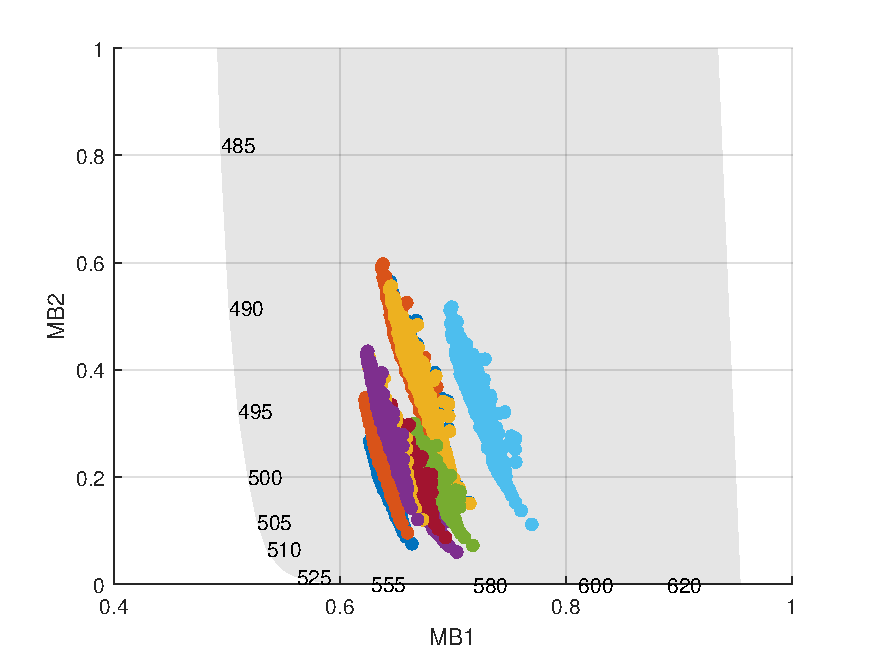
\includegraphics[width=\textwidth]{figs/mb.pdf}
%         \caption{$y=x$}
%         \label{fig:y equals x}
%     \end{subfigure}
%     \hfill
%     \begin{subfigure}[b]{0.49\textwidth}
%         \centering
%         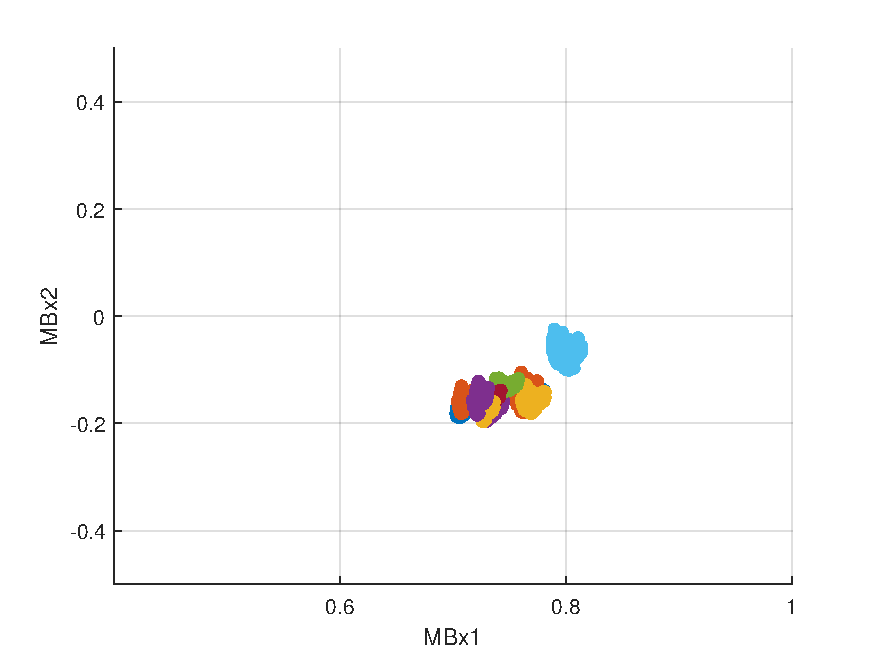
\includegraphics[width=\textwidth]{figs/corrected.pdf}
%         \caption{$y=3sinx$}
%         \label{fig:three sin x}
%     \end{subfigure}
%     \hfill
%        \caption{Three simple graphs}
%        \label{fig:three graphs}
%\end{figure}
